\chapter*{Figures}
\addcontentsline{toc}{chapter}{Figures}

The most notable figures are included in this list. They're high resolution thus zooming in the PDF should be viable to get a clearer view.

%------------------------------------

\section*{Data distribution of training set}
\addcontentsline{toc}{section}{Data distribution of training set}

\begin{figure}[H]
    \fbox{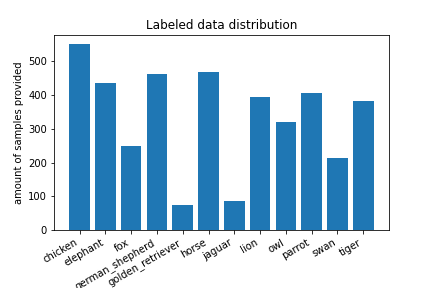
\includegraphics[width=1\linewidth]{images/1-data_analysis-labeled_data_distribution.png}}
    \captionsetup{width=0.85\linewidth}
    \captionsetup{justification=centering}
    \caption{The data distribution of the supplied training set.}
\end{figure}

%------------------------------------

\section*{Overview of training set}
\addcontentsline{toc}{section}{Overview of training set}

\begin{figure}[H]
    \fbox{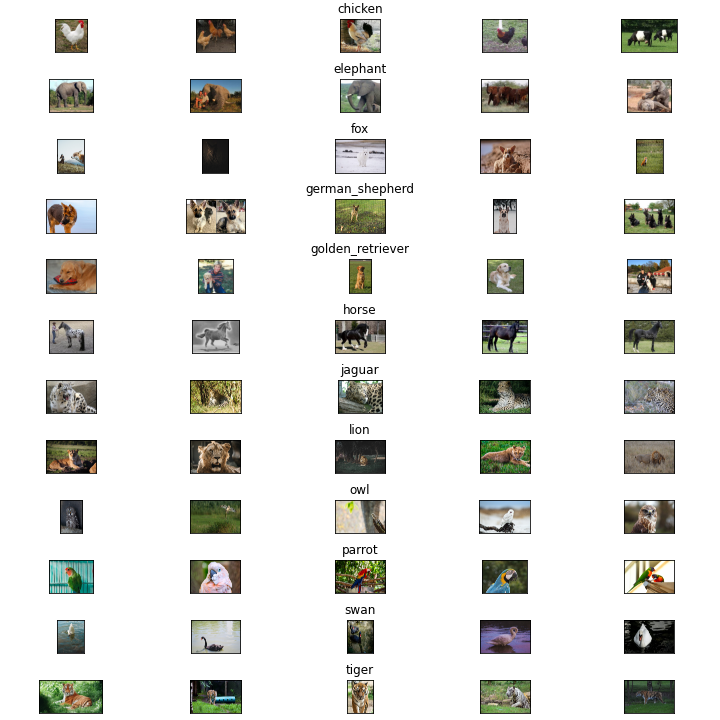
\includegraphics[width=1\linewidth]{images/1-data_analysis-labeled_data_overview.png}}
    \captionsetup{width=0.85\linewidth}
    \captionsetup{justification=centering}
    \caption{An overview of the supplied data per class.}
    \label{fig:1-data_analysis-labeled_data_overview.png}
\end{figure}

%------------------------------------

\section*{Shi-Tomasi corner detector example}
\addcontentsline{toc}{section}{Shi-Tomasi corner detector example}

\begin{figure}[H]
    \fbox{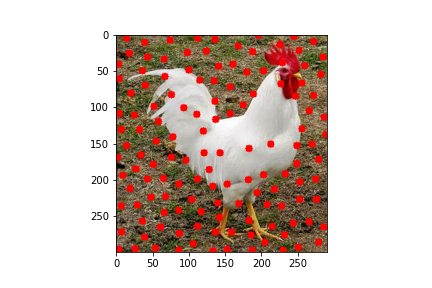
\includegraphics[width=1\linewidth]{images/1-data_analysis-POI.png}}
    \captionsetup{width=0.85\linewidth}
    \captionsetup{justification=centering}
    \caption{Example of points of interest found by Shi-Tomasi corner detector.}
\end{figure}

%------------------------------------

\section*{Overview of features data}
\addcontentsline{toc}{section}{Overview of features data}

\begin{figure}[H]
    \fbox{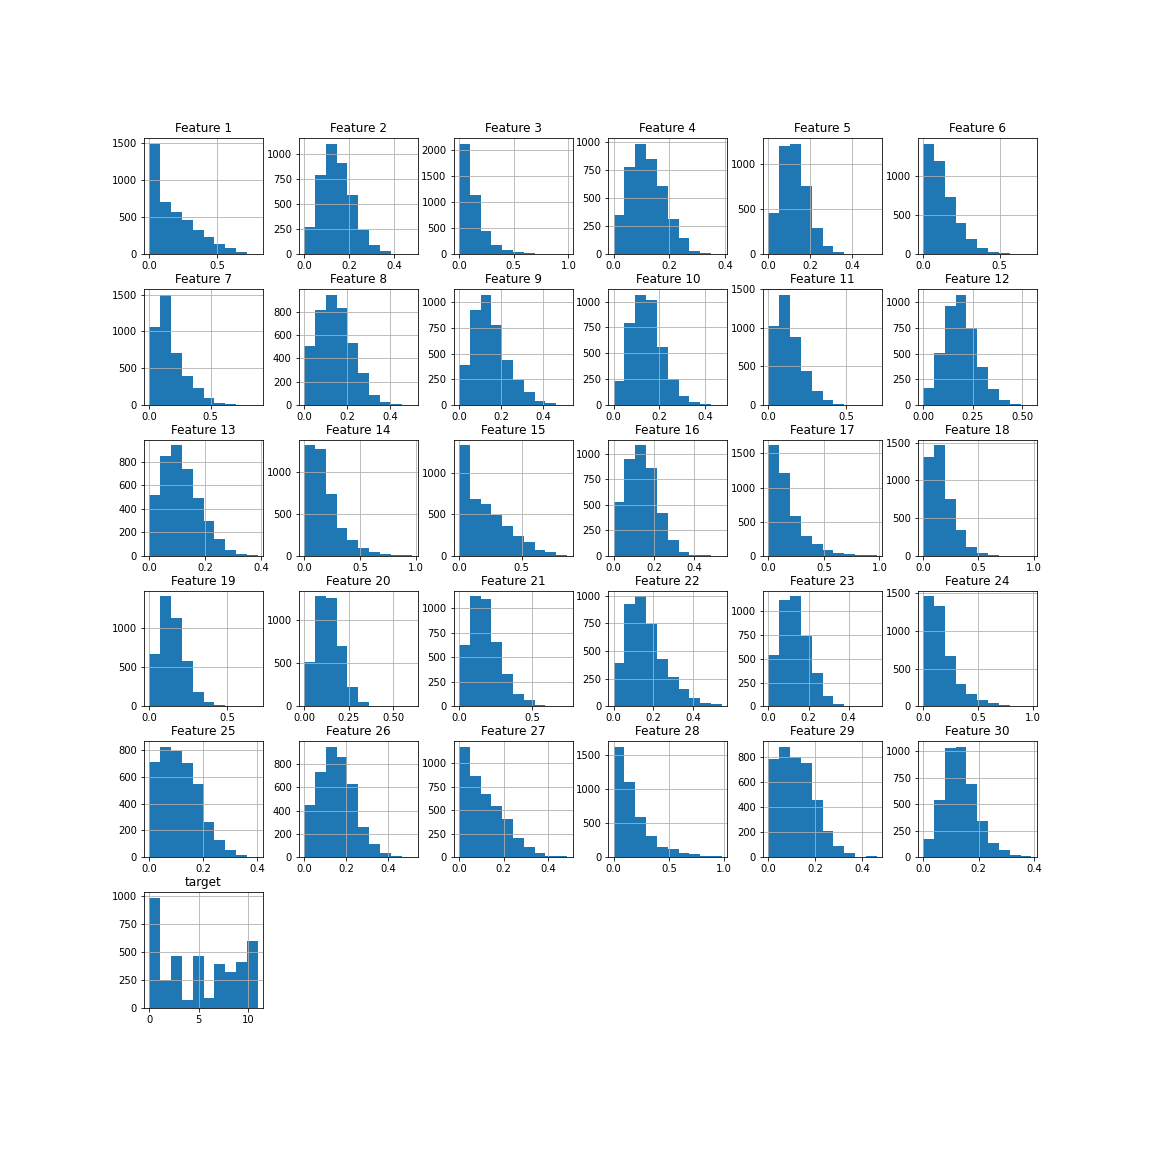
\includegraphics[width=1\linewidth]{images/1-data_analysis-feature_representation.png}}
    \captionsetup{width=0.85\linewidth}
    \captionsetup{justification=centering}
    \caption{An overview of the first 30 features data from a SIFT descriptor.}
    \label{fig:1-data_analysis-feature_representation}
\end{figure}